\documentclass[a4paper,12pt]{article}
\usepackage{tikz}
\usetikzlibrary{calc}
\begin{document}

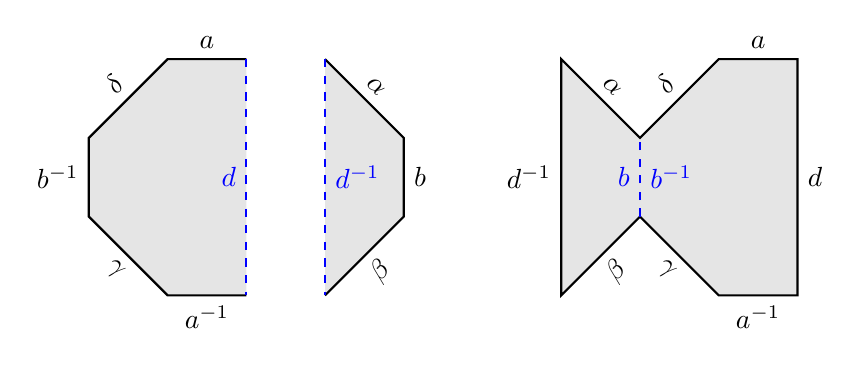
\begin{tikzpicture}[line width=0.8 pt]
\foreach \i in {-9,...,9}{
	\foreach \j in {-9,...,9}{
		\coordinate(v\i\j) at (\i,\j);
		\foreach \k in {1,...,8}{
			\coordinate(v\i\j\k) at ($(v\i\j)+(\k*45-22.5: 0.15)$);
		}
	}
}

\draw [fill=gray!20] (v20)--(v10)node[midway, below]{$a^{-1}$}--(v01)node[midway, sloped, below]{$\gamma$}--(v02)node[midway, left]{$b^{-1}$}--(v13)node[midway,sloped, above]{$\delta$}--(v23)node[midway,above]{$a$};
\draw [dashed, blue] (v23)--(v20)node[midway, left]{$d$};

\draw [fill=gray!20] (v33)--(v42)node[midway, sloped, above]{$\alpha$}--(v41)node[midway, right]{$b$}--(v30)node[midway,sloped, below]{$\beta$};
\draw [dashed, blue] (v33)--(v30)node[midway, right]{$d^{-1}$};


\draw [fill=gray!20] (v90)--(v80)node[midway, below]{$a^{-1}$}--(v71)node[midway, sloped, below]{$\gamma$}--(v60)node[midway,sloped, below]{$\beta$}--(v63)node[midway,left]{$d^{-1}$}--(v72)node[midway,sloped, above]{$\alpha$}--(v83)node[midway, sloped, above]{$\delta$}--(v93)node[midway, above]{$a$}--cycle node[midway, right]{$d$};
\draw [dashed, blue] (v71)--(v72)node[midway, left]{$b$}node[midway, right]{$b^{-1}$};

\end{tikzpicture}

\begin{center}
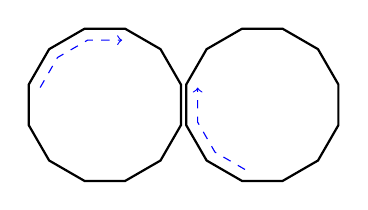
\begin{tikzpicture}[line width=0.8pt]
%\draw (0:0)--(0:1);
%\draw (0:0)--(45:1);
%\draw (0:0)--(90:1);
%\draw (0:0)--(135:1);
%\draw (0:0)--(180:1);
%\draw (0:0)--(225:1);
%\draw (0:0)--(270:1);
%\draw (0:0)--(315:1);

%draw options POSITION fonction ...
\foreach \k in {1,...,12}
{\coordinate(v\k) at ($(\k*30+15:1)+(-1,0)$);}
\foreach \k in {1,...,12}
{\coordinate(z\k) at ($(\k*30+15:1)+(1,0)$);}
\foreach \k in {1,...,12}
{\coordinate(w\k) at ($(\k*30+15:0.85)+(1,0)$);}

\foreach \k in {1,...,12}
{\coordinate(x\k) at ($(\k*30+15:0.85)+(-1,0)$);}
%\coordinate(v1) at (0:1);
%\coordinate(v2) at (45:1);
%\coordinate(v3) at (90:1);
%\coordinate(v4) at (135:1);
%\coordinate(v5) at (180:1);
%\coordinate(v6) at (225:1);
%\coordinate(v7) at (270:1);
%\coordinate(v8) at (315:1);
\draw [thin, dashed, blue, ->](w8)--(w7)--(w6)--(w5);
% Commence à angle 45 et rayon 0.85, va de rayon 45 à rayon 135
%\draw [thin, dashed,red!80, ->](w1) arc (30:90:0.85) node[below, midway]{$h_i$};

\draw [thin, dashed, blue, ->](x5)--(x4)--(x3)--(x2);
% On peut aussi enchaîner avec arc/circle...
\draw (v1)--(v2)--(v3)--(v4)--(v5)--(v6)--(v7)--(v8)--(v9)--(v10)--(v11)--(v12)--cycle;
\draw (z1)--(z2)--(z3)--(z4)--(z5)--(z6)--(z7)--(z8)--(z9)--(z10)--(z11)--(z12)--cycle;

\end{tikzpicture}
\end{center}

%\begin{center}
%\begin{tikzpicture}
%
%	\foreach \i [remember=\i as \j (initially 0), evaluate=\i as \c using 100*\i/100] in {10,20,...,100} {
%		%\fill [yellow!\c](\j:0.5) circle (0.5);
%		\fill [red!\c](\i:1) circle (0.5);
%		%\fill [blue!\c](-\j:0.5) circle (0.5);
%		\fill [black!\c](-\i:1) circle (0.5);
%	}
%\end{tikzpicture}
%\end{center}

\begin{center}
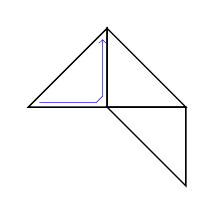
\begin{tikzpicture}[line width=0.5pt]
\foreach \i in {-9,...,9}{
	\foreach \j in {-9,...,9}{
		\coordinate(v\i\j) at (\i,\j);
		\foreach \k in {1,...,8}{
			\coordinate(v\i\j\k) at ($(v\i\j)+(\k*45-22.5: 0.15)$);
		}
	}
}

\draw (v00)--(v10)--(v11)--cycle;
\draw (v10)--(v20)--(v11)--cycle;
\draw (v10)--(v2-1)--(v20)--cycle;
\draw [line width=0.2pt, blue, ->] (v001)--(v104)--(v103)--(v116);

\end{tikzpicture}
\end{center}
\end{document}



